\documentclass[11pt]{article}
\usepackage{enumerate, graphicx, amsmath}
\usepackage[hidelinks]{hyperref}
\graphicspath{ {./img/} }
\parindent 0px
\date{\vspace{-10pt}\today}
\title{CS 362 :\hspace{2px}: Homework 3\\\Large{Karnaugh Maps}\vspace{-10pt}}
\author{Ryan Magdaleno}

% Helpful ::
% \line(1,0){358px}

\begin{document}
\maketitle

%%%%%%%%%%%%%%%%%%%%%%%%%%%%%%%%%%%%%%%%%%%%%%%%%%%%%%%%%%%%%%%%%%%%%%%%%%%%%%%%%%%%%%%%%

\vspace{-24pt}References used :\hspace{2pt}:
\href{https://www.youtube.com/watch?v=xGZeZOq-aRo}
{4-Input Karnaugh Maps (YouTube)}\vspace{10pt}

\textbf{Problem 1.} Find the simplified expression using the given the K-Maps. Note: the 
values in $m(\,\,\,)$ values are expression are where the minterms have a value of 1. 
Show your work.

\vspace{5px}\textbf{Solution ::}
\begin{enumerate}[a)]
    \item
    $F(A, B, C) = \Sigma m(0, 2, 3, 6)$
    \vspace{-15pt}\begin{center}
        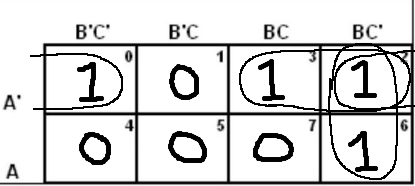
\includegraphics[scale=0.35]{1a.png}
    \end{center}
    \vspace{-20pt}\begin{enumerate}[$\bullet$]
        \item $A=0,\, B=1,\, C=$ 0 or 1
        \item \vspace{-5pt}$A=0,\,B = 0$ or $1,\, C=0$
        \item \vspace{-5pt}$A= 0$ or $1$, $B = 1,\,C=0$
    \end{enumerate}
    $$F(A,B,C) = A'B + A'C' + BC'$$
    \line(1,0){343px}

    \item
    $F(A, B, C) = \Sigma m(0, 1, 2, 4, 5)$
    \vspace{-15pt}\begin{center}
        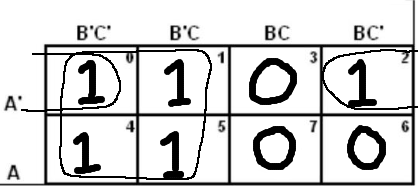
\includegraphics[scale=0.35]{1b.png}
    \end{center}
    \vspace{-20pt}\begin{enumerate}[$\bullet$]
        \item $A=0$ or $1,\, B=0,\, C=$ 0 or 1
        \item \vspace{-5pt}$A=0,\,B = 0$ or $1,\, C=0$
    \end{enumerate}
    $$F(A,B,C) = B' + A'C'$$
    \pagebreak

    \item
    $F(A, B, C) = \Sigma m(1,2,4,5,6,7)$
    \vspace{-15pt}\begin{center}
        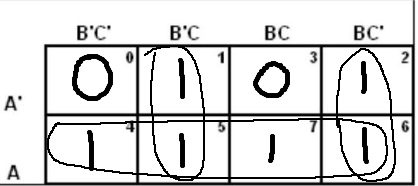
\includegraphics[scale=0.35]{1c.png}
    \end{center}
    \vspace{-20pt}\begin{enumerate}[$\bullet$]
        \item $A=1,\,B = 0$ or $1,\,C=0$ or $1$
        \item \vspace{-5pt}$A=0$ or $1,\,B=1,C=0$
        \item \vspace{-5pt}$A=0$ or $1,\,B=0,C=1$
    \end{enumerate}
    $$F(A,B,C) = A + BC' + B'C$$
\end{enumerate}

\pagebreak

%%%%%%%%%%%%%%%%%%%%%%%%%%%%%%%%%%%%%%%%%%%%%%%%%%%%%%%%%%%%%%%%%%%%%%%%%%%%%%%%%%%%%%%%%

\textbf{Problem 2.} Find the simplified expression using the given the K-Maps. Note: the 
values in $m(\,\,\,)$ values are expression are where the minterms have a value of 1. 
Show your work.

\vspace{5px}\textbf{Solution ::}
\begin{enumerate}[a)]
    \item
    $F(A,B,C,D) = \Sigma m(0,2,8,9,10,13)$
    \vspace{-15pt}\begin{center}
        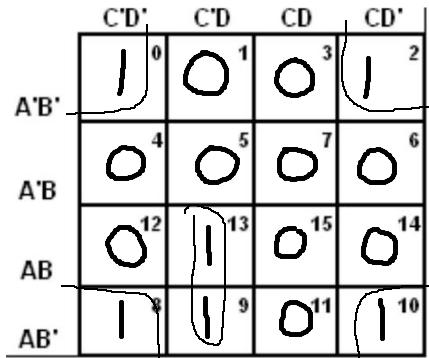
\includegraphics[scale=0.35]{2a.png}
    \end{center}
    \vspace{-20pt}\begin{enumerate}[$\bullet$]
        \item $A=0$ or $1,\,B=0,\,C=0$ or $1,\,D=0$
        \item \vspace{-5pt}$A=1,\,B=0$ or $1,\,C=0,\,D=1$
    \end{enumerate}
    $$F(A,B,C,D) = B'D' + AC'D$$
    \line(1,0){343px}

    \item
    $F(A,B,C,D) = \Sigma m(1,3,8,9,10,11,12,14)$
    \vspace{-15pt}\begin{center}
        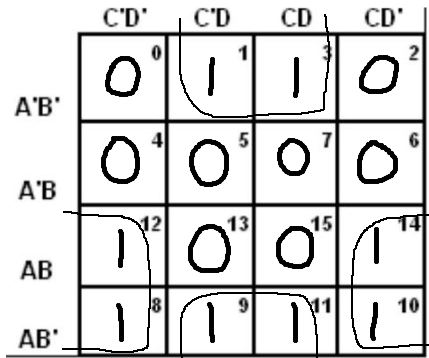
\includegraphics[scale=0.35]{2b.png}
    \end{center}
    \vspace{-20pt}\begin{enumerate}[$\bullet$]
        \item $A=0$ or $1,\,B=0,\,C=0$ or $1,\,D=1$
        \item \vspace{-5pt}$A=1,\,B=0$ or $1,\,C=0$ or $1,\,D=0$
    \end{enumerate}
    $$F(A,B,C,D) = B'D + AD'$$
    \pagebreak

    \item
    $F(A,B,C,D) = \Sigma m(3,4,5,11,13,15)$
    \vspace{-15pt}\begin{center}
        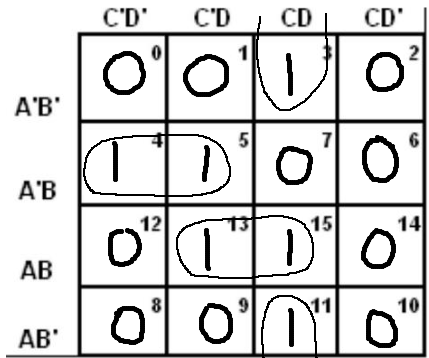
\includegraphics[scale=0.35]{2c.png}
    \end{center}
    \vspace{-20pt}\begin{enumerate}[$\bullet$]
        \item $A = 1,\, B = 1,\, C = 0$ or $1,\, D = 1$
        \item \vspace{-5pt}$A=0,\, B=1,\, C=0,\, D=0$ or $1$
        \item \vspace{-5pt}$A = 0$ or $1,\, B = 0,\, C = 1,\, D = 1$
    \end{enumerate}
    $$F(A,B,C,D) = ABD + A'BC' + B'CD$$
    \line(1,0){343px}

    \item
    $F(A,B,C,D) = \Sigma m(1,5,7,9,13,15)$
    \vspace{-15pt}\begin{center}
        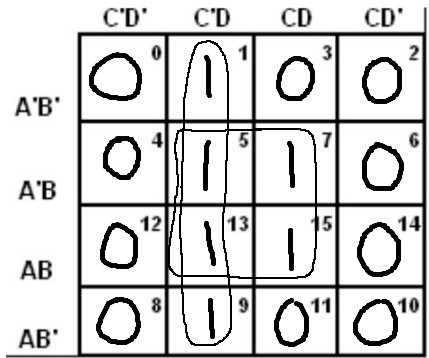
\includegraphics[scale=0.35]{2d.jpg}
    \end{center}
    \vspace{-20pt}\begin{enumerate}[$\bullet$]
        \item $A = 0$ or $1,\, B = 1,\, C = 0$ or $1,\, D = 1$
        \item \vspace{-5pt}$A = 0$ or $1,\, B = 0$ or $1,\, C = 0,\, D = 1$
    \end{enumerate}
    $$F(A,B,C,D) = BD + C'D$$
\end{enumerate}

\pagebreak

%%%%%%%%%%%%%%%%%%%%%%%%%%%%%%%%%%%%%%%%%%%%%%%%%%%%%%%%%%%%%%%%%%%%%%%%%%%%%%%%%%%%%%%%%

\textbf{Problem 3.} Find the simplified expression using the given the K-Maps. Note: the 
values in $m(\,\,\,)$ values are expression are where the minterms have a value of 1.
The $d(\,\,\,)$ values are where the minterms are “don’t care” conditions. 
Show your work.

\vspace{5px}\textbf{Solution ::}
\begin{enumerate}[a)]
    \item 
    $F(A,B,C,D) = \Sigma m(1,5,7,11) + \Sigma d(3,4,13,14)$
    \vspace{-15pt}\begin{center}
        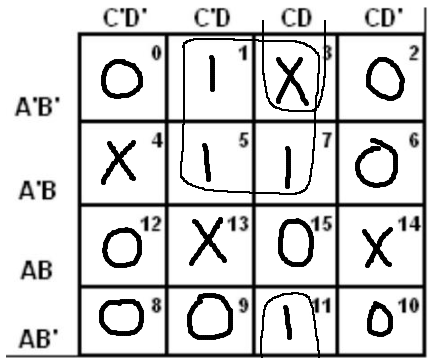
\includegraphics[scale=0.35]{3a.png}
    \end{center}
    \vspace{-20pt}\begin{enumerate}[$\bullet$]
        \item $A = 0,\, B = 0$ or $1,\, C = 0$ or $1,\, D = 1$
        \item \vspace{-5pt}$A = 0$ or $1,\, B = 0,\, C = 1,\, D = 1$
    \end{enumerate}
    $$F(A,B,C,D) = A'D + B'CD$$
    \line(1,0){343px}

    \item 
    $F(A,B,C,D) = \Sigma m(1,4,8,9,11,13) + \Sigma d(7,10,12,14,15)$
    \vspace{-15pt}\begin{center}
        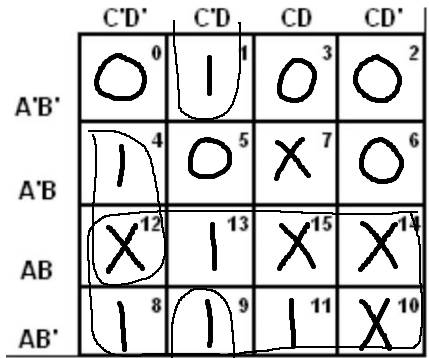
\includegraphics[scale=0.35]{3b.png}
    \end{center}
    \vspace{-20pt}\begin{enumerate}[$\bullet$]
        \item $A = 0$ or $1,\, B = 1,\, C = 0,\, D = 0$
        \item \vspace{-5pt}$A = 0$ or $1,\, B = 0,\, C = 0,\, D = 1$
        \item \vspace{-5pt}$A = 1,\, B = 0$ or $1,\, C = 0$ or $1,\, D = 0$ or $1$
    \end{enumerate}
    $$F(A,B,C,D) = BC'D' + B'C'D + A$$
    \pagebreak

    \item 
    $F(A,B,C,D) = \Sigma m(5,9,12,14) + \Sigma d(3,6,8,11,13,15)$
    \vspace{-15pt}\begin{center}
        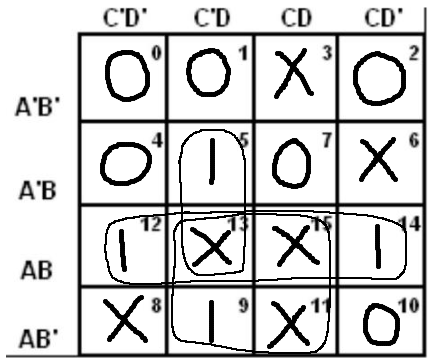
\includegraphics[scale=0.35]{3c.png}
    \end{center}
    \vspace{-20pt}\begin{enumerate}[$\bullet$]
        \item $A = 1,\, B = 0$ or $1,\, C = 0$ or $1,\, D = 1$
        \item \vspace{-5pt}$A = 1,\, B = 1,\, C = 0$ or $1,\, D = 0$ or $1$
        \item \vspace{-5pt}$A = 0$ or $1,\, B = 1,\, C = 0,\, D = 1$
    \end{enumerate}
    $$F(A,B,C,D) = AD + AB + BC'D$$

\end{enumerate}
\end{document}